% Chapter 4

\chapter{EXPERIMENTAL RESULTS AND PERFORMANCE ANALYSIS}\label{cha:results}

This chapter contains the information that forms the basis of the system, both the
hardware and software, the experiments carried out thus far, and the conclusions made
from them. The quantitative results come from four different places: the first run of
the evaluation loop (refer Section~\ref{sec:m5}), wind experiment, the ablation runner,
and the very first SITL flights. They are
preliminary in a specific sense: MOPSO was run at reduced settings, the risk weights and
battery constants are not yet calibrated, and the synthetic density labels have a known
defect. Each caveat is stated next to the result it affects.

\section{DATASET DESCRIPTION}\label{sec:dataset}

The datasets of the works we reviewed are custom or not released, so, as is common in
this field, we built our own environments. There are two kinds: synthetic airspace graphs, generated from fixed seeds, for
controlled benchmarks; and a real-region lattice built from public geographic and
weather data. Table~\ref{tab:datasets} lists every graph used in this chapter.

\begin{table}[!htbp]
\centering
\caption{Graphs and scenarios used in the experiments}\label{tab:datasets}
\small
\begin{tabular}{|P{3.0cm}|P{2.9cm}|P{8.3cm}|}
\hline
\textbf{Scenario} & \textbf{Size} & \textbf{Description}\\
\hline
S1 small sparse & 50 nodes & Synthetic grid, seed 101, 5\% obstacle coverage label, weather seeded\\
\hline
S2 medium & 196--200 nodes & Synthetic grid, seed 202, 20\% label; weather seeded (benchmark) or set explicitly (wind experiment)\\
\hline
S3 large dense & 500 nodes & Synthetic grid, seed 303, 40\% label, weather seeded\\
\hline
Real-region lattice & 893 nodes, 6,752 edges & 6\,km box, 200\,m spacing, offline fixture layers (ablation)\\
\hline
Small lattice & 2\,km box, 200\,m spacing & Lattice used for the route figure in Section~\ref{sec:perf-tier2}\\
\hline
Flat lattice & 225 nodes, 1,624 edges & 3\,km box, 200\,m spacing, no layers (directional cost check)\\
\hline
Simulation bundle & 1.5\,km box, 100\,m lattice & Frozen terrain, buildings, roads and pads for Gazebo and SITL\\
\hline
\end{tabular}
\end{table}

\subsection{Synthetic airspace graphs}

The synthetic graphs come from the seeded builder of Section~\ref{sec:m1}. Each is a
jittered grid of about 1.3\,km spacing with 8-neighbour directed edges, seeded Gaussian
hills for terrain, obstacle discs, and seeded wind between 12 and 28\,km/h with a gust
factor of 1.4. The three scales (50, 200 and 500 nodes) were chosen to cover a sanity
check, a mid-sized core case and a stress case. Every draw comes from the seed, so the graphs are reproducible.

There is one known defect in this data. The density obstacle labels (5\%, 20\% and
40\%) do not affect the graph builder at all; rather, the benchmark runner rescales the
end risk value. As a result, the scenarios vary in size and seeds and not in obstacle
density regardless of the labels. This is corrected in the next pass, and all benchmark
values are recalculated.

\subsection{Real-region lattice}

Four public data sources feed the real-region lattice (Table~\ref{tab:sources}).
Nothing in the method ties it to one place; our example is a coastal urban
neighbourhood. The default 6\,km box at 200\,m spacing has 900 candidate nodes, of which 893 remain after node selection and connectivity pruning in the fixture run, linked by
6,752 directed edges.

\begin{table}[!htbp]
\centering
\caption{Environment data sources for the real-region lattice}\label{tab:sources}
\small
\begin{tabular}{|P{2.8cm}|P{4.3cm}|P{7.1cm}|}
\hline
\textbf{Layer} & \textbf{Source} & \textbf{Used for}\\
\hline
Weather & Open-Meteo forecast~\cite{r20} & Wind speed and direction at 10\,m and 80\,m, gust, rain, visibility, WMO code\\
\hline
Terrain & Local GeoTIFF, OpenTopography Copernicus 30\,m, Open-Meteo elevation (Copernicus 90\,m), flat fallback & Ground elevation of nodes and edge samples\\
\hline
Buildings & OpenStreetMap via Overpass & Footprints and heights; node altitude, building risk, density, turbulence, urban canyon\\
\hline
Restricted zones & OpenStreetMap via Overpass & Aerodromes, military land, prisons, protected areas, government sites; node and edge removal, soft buffer\\
\hline
Water and land use & OpenStreetMap via Overpass, coastline & Water fraction, population exposure classes, major roads\\
\hline
\end{tabular}
\end{table}

Public Overpass server sometimes resets or times out. For the offline and replicable
experiments, the project offers fixture layers that represent manually created test data
mimicking the real region. The ablation from Section~\ref{sec:perf-ablation} was done
using such fixtures showing how each layer affects the planner rather than providing
metrics available in reality.

\subsection{Payload tag space and simulation bundle}

We evaluate Tier~2 on all 225 tag combinations. Four reference presets
(Table~\ref{tab:presets}) stand in for deliveries led by risk, by distance and by
energy, and one balanced delivery. For simulation we freeze a 1.5\,km region into a
bundle, and its hash binds the planner graph, stored front, mission file and Gazebo
world to each other.

\section{ECOSYSTEM}\label{sec:ecosystem}

\subsection{Hardware configuration}

All planner experiments in this chapter ran on a laptop-class CPU without a GPU. The
planner does not need one: Tier~1 is a graph search that runs on a single core, and
Tier~2 is a closed-form computation. The simulation runs under WSL2 (Ubuntu 24.04) on
the same class of machine.

Phase~II moves the system onto standard, commercially available hardware: an F450
quadcopter frame with a Pixhawk flight controller running ArduCopter, a Raspberry Pi~5
companion computer that hosts Tier~2 on board, a servo payload release and a MAVLink
telemetry link to the ground station.

\subsection{Software environment}

All code is written in Python~3. NetworkX~\cite{r5} holds the directed airspace
graph and runs the A* baselines; NumPy handles dominance checks and metrics; Shapely~2
STRtree indexes hold the spatial layers; and GeoPandas, pyogrio and OSMnx~\cite{r4}
parse and cache the OpenStreetMap layers. Figures use Matplotlib, the dashboard
Tkinter, and the offline test suites unittest. Simulation uses Gazebo
Harmonic~\cite{r24}, ArduPilot SITL~\cite{r23}, pymavlink over MAVLink~\cite{r7} and
QGroundControl.

\section{EXPERIMENTS CONDUCTED}\label{sec:experiments}

Table~\ref{tab:experiments} summarises the experiments. Each is described below, and
Section~\ref{sec:performance} analyses the results.

\begin{table}[!htbp]
\centering
\caption{Experiments carried out in Phase~I so far}\label{tab:experiments}
\small
\begin{tabular}{|P{0.7cm}|P{3.5cm}|P{3.2cm}|P{6.6cm}|}
\hline
\textbf{No.} & \textbf{Experiment} & \textbf{Data} & \textbf{Question}\\
\hline
E1 & Front quality benchmark & S1, S2, S3 & Does the exact Tier~1 front beat single-objective A* and MOPSO on HV, IGD and spread, and at what runtime cost?\\
\hline
E2 & Wind direction study & S2 under calm air and 8 directions; 15$^\circ$ sweep & How much does wind direction alone change the front and the Tier~2 picks?\\
\hline
E3 & Directional edge costs & Flat lattice, wind from the east & Do edge costs respond to heading as the model predicts?\\
\hline
E4 & Risk-layer ablation & Real-region lattice, fixture layers & Which layers drive risk, energy and front size?\\
\hline
E5 & Tier~2 selection & S2, S3 and small lattice fronts & Do different payloads get different routes, including non-extreme ones, within 1\,s?\\
\hline
E6 & SITL flights & Fixture bundle, ArduCopter SITL & Is the mission chain from Tier~2 to the autopilot correct?\\
\hline
E7 & Automated tests & Planner and simulation suites & Do the components behave as specified?\\
\hline
\end{tabular}
\end{table}

The settings were as follows. In E1, all methods used the same source and target per
scenario, and HV, IGD and spread were computed against the union reference front. MOPSO
ran at a reduced setting of 24 particles, 30 iterations and 2 repetitions per scenario
to get a complete first pass quickly; the report-scale run (100, 200 and 30) is the next
step. In E2, the S2 graph (196 nodes, 1,404 edges, seed 202) was costed under calm air
and under a 25\,km/h wind with 35\,km/h gusts from each of eight compass directions, then
in 15$^\circ$ steps, with the graph, layers, source and target unchanged. E3 used a flat
3\,km lattice with no terrain, buildings or zones under a 25\,km/h east wind. E4 rebuilt
the real-region front with all layers, without wind, without terrain and without
buildings, under a 30\,km/h wind from the south-west. E5 ran the four presets on the S2
front (16 routes), the S3 front (115 routes) and a 2\,km lattice. E6 flew planner
missions from a fixture bundle against ArduCopter SITL (4.8.0-dev, built-in quadcopter
physics, five times real time), and a Tier~2 mission was also flown in the Gazebo city
world. E7 covers about 220 planner tests and 45 simulation tests, all offline;
Appendix~\ref{app:tests} lists them. One of them compares the NAMOA* front with a
brute-force front over all simple paths on a small graph, which is our strongest check
that Tier~1 is exact.

\section{PERFORMANCE ANALYSIS}\label{sec:performance}

\subsection{Tier 1 front quality against the baselines}\label{sec:perf-front}

The first-pass benchmark is in Table~\ref{tab:bench}.

\begin{table}[!htbp]
\centering
\caption{First-pass benchmark on the synthetic scenarios (HV higher is better; IGD and
$\Delta$ lower are better)}\label{tab:bench}
\small
\begin{tabular}{|l|l|r|r|r|r|r|}
\hline
\textbf{Scenario} & \textbf{Method} & \textbf{Front} & \textbf{Time (s)} & \textbf{HV} & \textbf{IGD} & $\boldsymbol{\Delta}$\\
\hline
\multirow{5}{*}{S1 (50)} & NAMOA* (Tier 1) & 2 & 0.003 & 0.131 & 0.000 & 0.000\\
 & A* distance & 1 & $<$0.001 & 0.121 & 0.866 & --\\
 & A* energy & 1 & $<$0.001 & 0.121 & 0.866 & --\\
 & A* risk & 1 & $<$0.001 & 0.011 & 0.866 & --\\
 & MOPSO & 2 & 0.363 & 0.131 & 0.000 & 0.000\\
\hline
\multirow{5}{*}{S2 (200)} & NAMOA* (Tier 1) & 16 & 0.162 & 1.2065 & 0.000 & 1.001\\
 & A* distance & 1 & $<$0.001 & 0.107 & 1.021 & --\\
 & A* energy & 1 & $<$0.001 & 1.083 & 0.648 & --\\
 & A* risk & 1 & $<$0.001 & 0.011 & 0.887 & --\\
 & MOPSO & 12 & 1.505 & 1.2061 & 0.017 & 1.027\\
\hline
\multirow{5}{*}{S3 (500)} & NAMOA* (Tier 1) & 115 & 33.761 & 1.1235 & 0.000 & 0.666\\
 & A* distance & 1 & 0.001 & 0.062 & 0.861 & --\\
 & A* energy & 1 & 0.002 & 0.674 & 0.442 & --\\
 & A* risk & 1 & 0.002 & 0.013 & 1.116 & --\\
 & MOPSO & 38 & 4.326 & 1.1146 & 0.043 & 0.814\\
\hline
\end{tabular}
\end{table}

NAMOA* achieves a perfect zero inverted generational distance (IGD) for all three cases,
with all reference points found on the front of NAMOA*. This is the best that can be
achieved by an exact algorithm and indicates clearly that no solution is lost through
pruning rules. MOPSO recovers 12 of the 16 routes
on S2 and 38 of the 115 on S3, and its HV is close to that of NAMOA*, with a gap of
0.0004 on S2 and 0.009 on S3.

The HV gap is small because MOPSO's archive still reaches the extremes of the front
while missing most interior points, and interior points are the ones Tier~2 needs for
mixed payloads. For this project the IGD and front-size columns say more than HV. NAMOA* also spreads its points more
evenly, with $\Delta$ of 0.666 against 0.814 on S3. On S1 both methods find the same
two-route front, which tells us the smallest scenario is too easy to separate them.

The single-objective A* routes reach a high HV only when their one objective happens to
dominate the volume, as A* energy does on S2. None of them can cover the front, and their
IGD stays between 0.44 and 1.12. Figure~\ref{fig:bench-hv} plots HV per method.

\begin{figure}[!htbp]
\centering
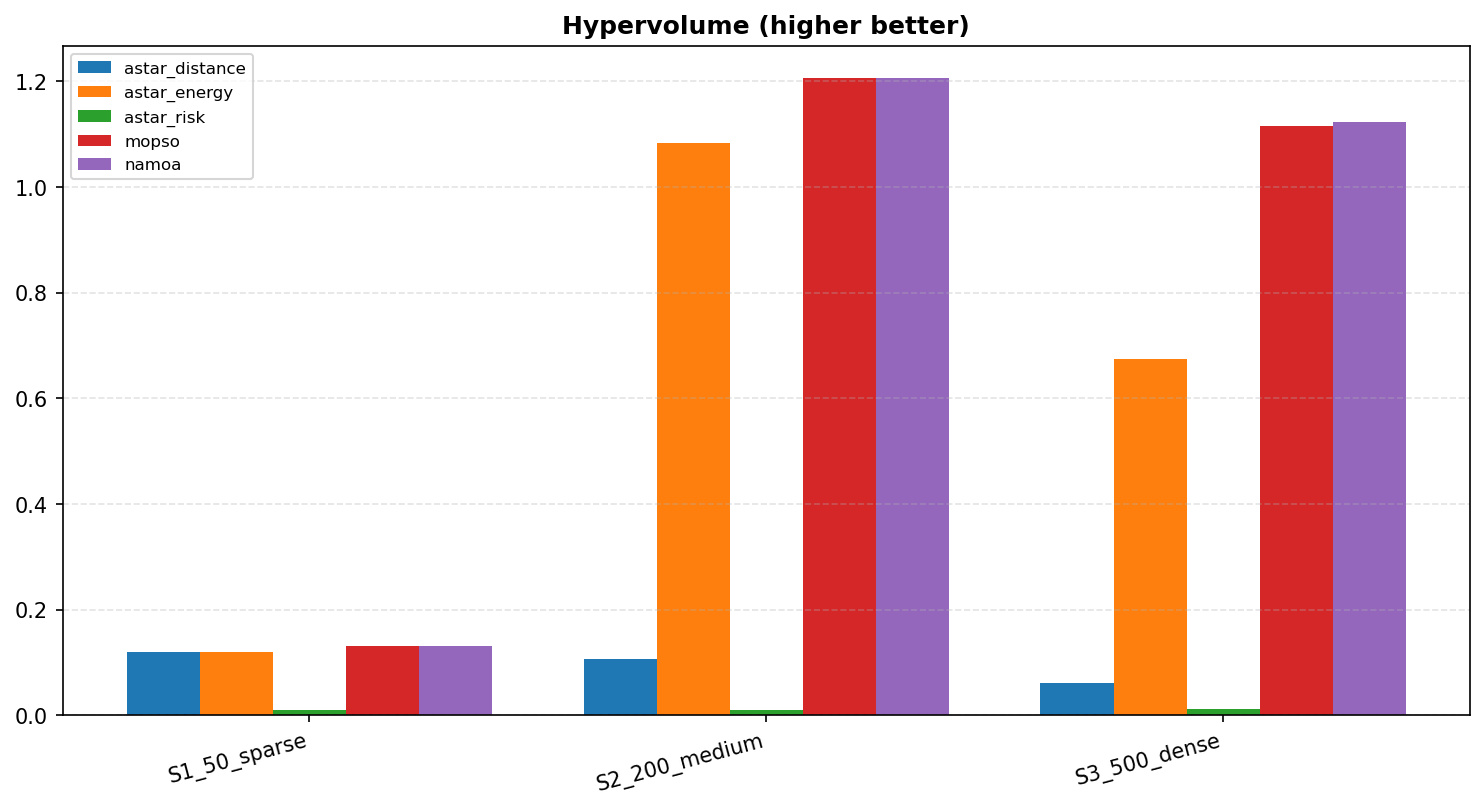
\includegraphics[width=0.62\textwidth]{images/benchmark_hv.jpg}
\caption{Hypervolume per method and scenario (first pass)}\label{fig:bench-hv}
\end{figure}

Exactness has a price. On S3, NAMOA* took 33.8\,s against 4.3\,s for MOPSO, and the
runtime grows quickly with front size. Tier~1 runs once per region and weather window,
not once per mission, so half a minute is acceptable, but it is still the main
performance target for the next pass.

On S2 the HV values of 1.2065 and 1.2061 are too close to claim superiority without
the 30 seeded MOPSO repetitions and a statistical test, which the next pass will run.
The IGD result does not have this problem, since an IGD of zero cannot be beaten.

\subsection{Effect of wind speed and direction}\label{sec:res-wind}

Table~\ref{tab:wind} shows the result of experiment E2.

\begin{table}[!htbp]
\centering
\caption{Effect of wind direction on the S2 front (25\,km/h wind, 35\,km/h gust)}\label{tab:wind}
\footnotesize
\begin{tabular}{|l|r|r|r|r|c|r|}
\hline
\textbf{Wind from} & \textbf{Front} & \textbf{Labels} & \textbf{Min $\boldsymbol{\varepsilon}$} & \textbf{Min $\boldsymbol{\rho}$} & \textbf{Fragile pick $(d, \varepsilon, \rho)$} & \textbf{Distinct}\\
\hline
Calm & 36 & 869 & 24.41 & 0.07 & (26.78, 26.92, 0.11) & 4\\
\hline
0$^\circ$ (N) & 14 & 1019 & 31.01 & 3.24 & (26.16, 32.82, 3.40) & 2\\
\hline
45$^\circ$ (NE) & 6 & 545 & 31.34 & 1.89 & (26.16, 33.63, 1.89) & 2\\
\hline
90$^\circ$ (E) & 11 & 876 & 30.94 & 3.31 & (26.16, 32.75, 3.45) & 2\\
\hline
135$^\circ$ (SE) & 14 & 1100 & 27.13 & 4.27 & (26.16, 29.59, 4.42) & 2\\
\hline
180$^\circ$ (S) & 14 & 989 & 26.18 & 3.24 & (26.16, 27.99, 3.40) & 2\\
\hline
225$^\circ$ (SW) & 6 & 482 & 24.58 & 1.89 & (26.16, 26.87, 1.89) & 2\\
\hline
270$^\circ$ (W) & 11 & 801 & 26.22 & 3.31 & (26.16, 28.03, 3.45) & 2\\
\hline
315$^\circ$ (NW) & 14 & 1084 & 27.21 & 4.27 & (26.16, 29.67, 4.42) & 2\\
\hline
\end{tabular}
\end{table}

The first observation is that direction alone matters a great deal. At the same speed,
the cheapest route on the front needs 24.58 energy units with the wind from the
south-west and 31.34 with it from the north-east, a difference of 27.5\%. A planning
algorithm using wind speed independent of its direction will cost both situations
equally.

The two goals depend on different criteria. When the wind is rotated 180$^\circ$ (from
0$^\circ$ to 180$^\circ$ or from 45$^\circ$ to 225$^\circ$), the lowest risk remains the
same because of the crosswind, which depends only on the wind's axis. Minimum energy
cannot be considered separately from the direction of the wind: the headwind cost is
conditional on the direction of the movement of the drone with respect to the relevant
axis. Both of them derive from Equation~(\ref{eq:hwcw}), which explains why headwind and
crosswind are two separate cases.

The pattern of the front also depends on the state of the wind. In calm conditions, 36
routes are possible; under 8 wind directions, the number of available routes is 6--14,
while the four presets give rise to just two unique routes. The reasoning here is that
in wind, highly crosswind-unfavorable edges become not only expensive but risky, leading
to a coincidence of costs and risks. The most sensitive case -- fragile medical pick --
always provides the safest path in wind, although the energy consumption of the route is
wind-dependent (26.87--33.63). Repeating the run in 15$^\circ$ steps (Figure~\ref{fig:wind-sweep}) gives a
minimum energy of 24.6 to 31.6 units, a 28.5\% swing, with 6 to 15 routes on the front.

\begin{figure}[!htbp]
\centering
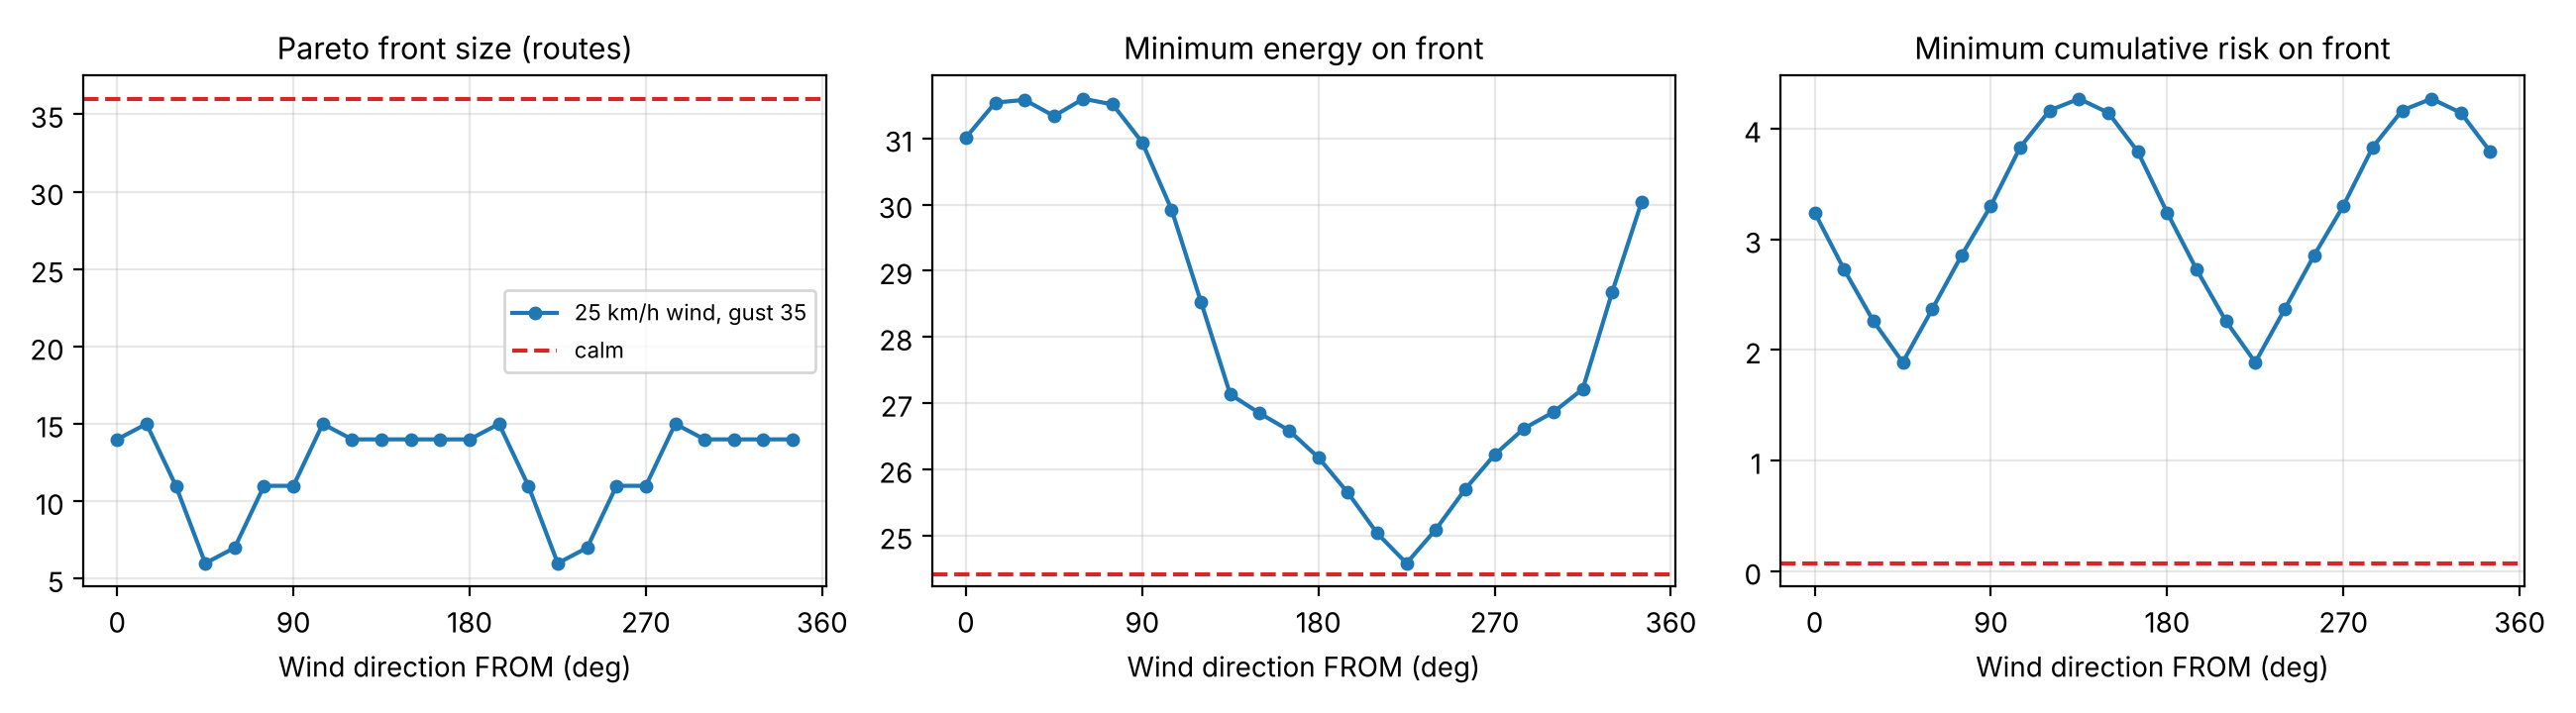
\includegraphics[width=0.9\textwidth]{images/wind_direction_sweep.jpg}
\caption{Front size, minimum energy and minimum risk on S2 as a 25\,km/h wind turns
through 360$^\circ$; the dashed line is calm air}\label{fig:wind-sweep}
\end{figure}

The collapse from four distinct picks to two may be the right answer for a front with
fewer real trade-offs, or a side effect of min-max normalisation on a short front. The
next pass will test both, and the answer may change Tier~2.

\subsection{Directional edge costs}

Table~\ref{tab:dir-edges} gives the result of E3.

\begin{table}[!htbp]
\centering
\caption{Directional edge costs on a flat lattice, 25\,km/h wind from 90$^\circ$}\label{tab:dir-edges}
\small
\begin{tabular}{|l|r|r|r|r|r|r|r|r|}
\hline
\textbf{Edge heading} & 0$^\circ$ & 45$^\circ$ & 90$^\circ$ & 135$^\circ$ & 180$^\circ$ & 225$^\circ$ & 270$^\circ$ & 315$^\circ$\\
\hline
$\varepsilon / d$ & 1.104 & 1.270 & 1.278 & 1.270 & 1.104 & 1.074 & 1.000 & 1.074\\
\hline
$\rho_\mathrm{edge}$ & 0.225 & 0.170 & 0.038 & 0.170 & 0.225 & 0.170 & 0.038 & 0.170\\
\hline
\end{tabular}
\end{table}

Flying east, into the wind, costs 27.8\% more energy per kilometre than flying west,
which costs exactly the distance because a tailwind earns no credit. For north and south
facing edges, the entire crosswind is present, and the risk score is six times that of
east-west edges (0.225 compared to 0.038). The value of 0.038 is only that of the gust
term for east-west edges. Still, the front on the flat lattice has only one route, as the straight diagonal is best for all goals. There is no trade-off resulting from the wind alone.

\subsection{Contribution of each risk layer}\label{sec:perf-ablation}

E4 test results are tabulated in Table~\ref{tab:ablation}. The experiments used fixture layers, so the values show how the layers affect the planner.

\begin{table}[!htbp]
\centering
\caption{Ablation on the 6\,km lattice (fixture layers, 30\,km/h wind from 225$^\circ$)}\label{tab:ablation}
\small
\begin{tabular}{|l|r|r|r|r|r|r|}
\hline
\textbf{Variant} & \textbf{Front} & \textbf{Time (s)} & \textbf{Min $\boldsymbol{\varepsilon}$} & \textbf{Min $\boldsymbol{\rho}$} & \textbf{Max $\boldsymbol{\rho}$} & \textbf{Mean $\boldsymbol{\rho_\mathrm{edge}}$}\\
\hline
All layers & 196 & 11.35 & 8.82 & 8.85 & 13.12 & 0.199\\
\hline
No wind & 205 & 5.38 & 7.84 & 0.10 & 4.24 & 0.061\\
\hline
No terrain & 56 & 1.36 & 8.81 & 8.81 & 13.08 & 0.198\\
\hline
No buildings & 190 & 8.32 & 8.82 & 8.85 & 12.26 & 0.192\\
\hline
\end{tabular}
\end{table}

Wind matters most here: turning it off lowers the mean edge risk
from 0.199 to 0.061, the safest path risk from 8.85 to 0.10, and the minimum energy by
11\%. Terrain, on the other hand, mostly controls how many routes there are. Without
grades there are far fewer distinct trade-offs, 56 routes against 196, because altitude
changes are what separate otherwise similar paths. Buildings raise the top limit of the
risk range.

\subsection{Tier 2 selection}\label{sec:perf-tier2}

Table~\ref{tab:tier2} gives the Tier~2 picks of E5 on the S2 and S3 fronts. The ranks
are the selected route's position on each objective within the front, where 1 is best.

\begin{table}[!htbp]
\centering
\caption{Tier~2 picks on the S2 (16 routes) and S3 (115 routes) fronts}\label{tab:tier2}
\footnotesize
\begin{tabular}{|l|l|r|r|r|r|r|r|l|r|}
\hline
\textbf{Front} & \textbf{Preset} & $\boldsymbol{d}$ & $\boldsymbol{\varepsilon}$ & $\boldsymbol{\rho}$ & \textbf{Rk $d$} & \textbf{Rk $\varepsilon$} & \textbf{Rk $\rho$} & \textbf{Point type} & \textbf{ms}\\
\hline
\multirow{4}{*}{S2} & Fragile medical & 19.45 & 20.94 & 0.69 & 7 & 5 & 10 & non-extreme & 0.030\\
 & Emergency medicine & 19.15 & 20.56 & 0.81 & 3 & 1 & 14 & min-energy & 0.025\\
 & Disaster relief & 19.15 & 20.56 & 0.81 & 3 & 1 & 14 & min-energy & 0.022\\
 & Mixed cargo & 19.22 & 20.66 & 0.75 & 4 & 2 & 13 & non-extreme & 0.023\\
\hline
\multirow{4}{*}{S3} & Fragile medical & 41.02 & 45.86 & 1.92 & 91 & 81 & 25 & non-extreme & 0.144\\
 & Emergency medicine & 37.11 & 44.71 & 6.56 & 22 & 26 & 94 & non-extreme & 0.140\\
 & Disaster relief & 37.52 & 44.27 & 5.63 & 28 & 1 & 88 & min-energy & 0.136\\
 & Mixed cargo & 39.90 & 45.06 & 2.74 & 84 & 59 & 32 & non-extreme & 0.136\\
\hline
\end{tabular}
\end{table}

On the 115-route S3 front, the four presets take four separate routes, three of which are represented by non-extreme points. Disaster relief uses the minimum energy path, consistent with its dominant weight.

The emergency medicine preset deserves a special consideration. It is merely the
22nd shortest route, yet it is just 1.9\% longer than the shortest route in the front.
While the distance is the key factor in the setting of its weights, it is not the only
one; therefore, the utility function sacrifices some distance for smaller risk. A single
objective planner cannot do that kind of tradeoff, and a fixed weights planner would
make the same tradeoff for each payload.

The fragile medical and emergency routes show the gap between Tier~2 options. The fragile route is 10.5\% longer than the emergency one
(41.02 versus 37.11), and it has 71\% less risk (1.92 versus 6.56). It ranks 25th out of
115 on risk instead of 1st, because both distance and energy coefficients are still positive and the more cautious paths are much longer.
Mixed cargo is in an intermediate position with respect to all criteria, as expected from its balanced weights. Selections on S3
took about 0.14\,ms, against a target of one second.

On the smaller S2 front, emergency medicine and disaster relief take the same minimal energy path, as in the wind example: small fronts leave Tier~2 fewer paths.

Figure~\ref{fig:osm-routes} shows the four presets on a 2\,km lattice (11-route front) with
OpenStreetMap roads drawn underneath for reference. The fragile medical and mixed cargo
presets take a slightly longer path (2.6\,km) with a cumulative risk of 1.57, while
emergency medicine and disaster relief take 2.5\,km paths with risks of 1.88 and 1.89.

\begin{figure}[!htbp]
\centering
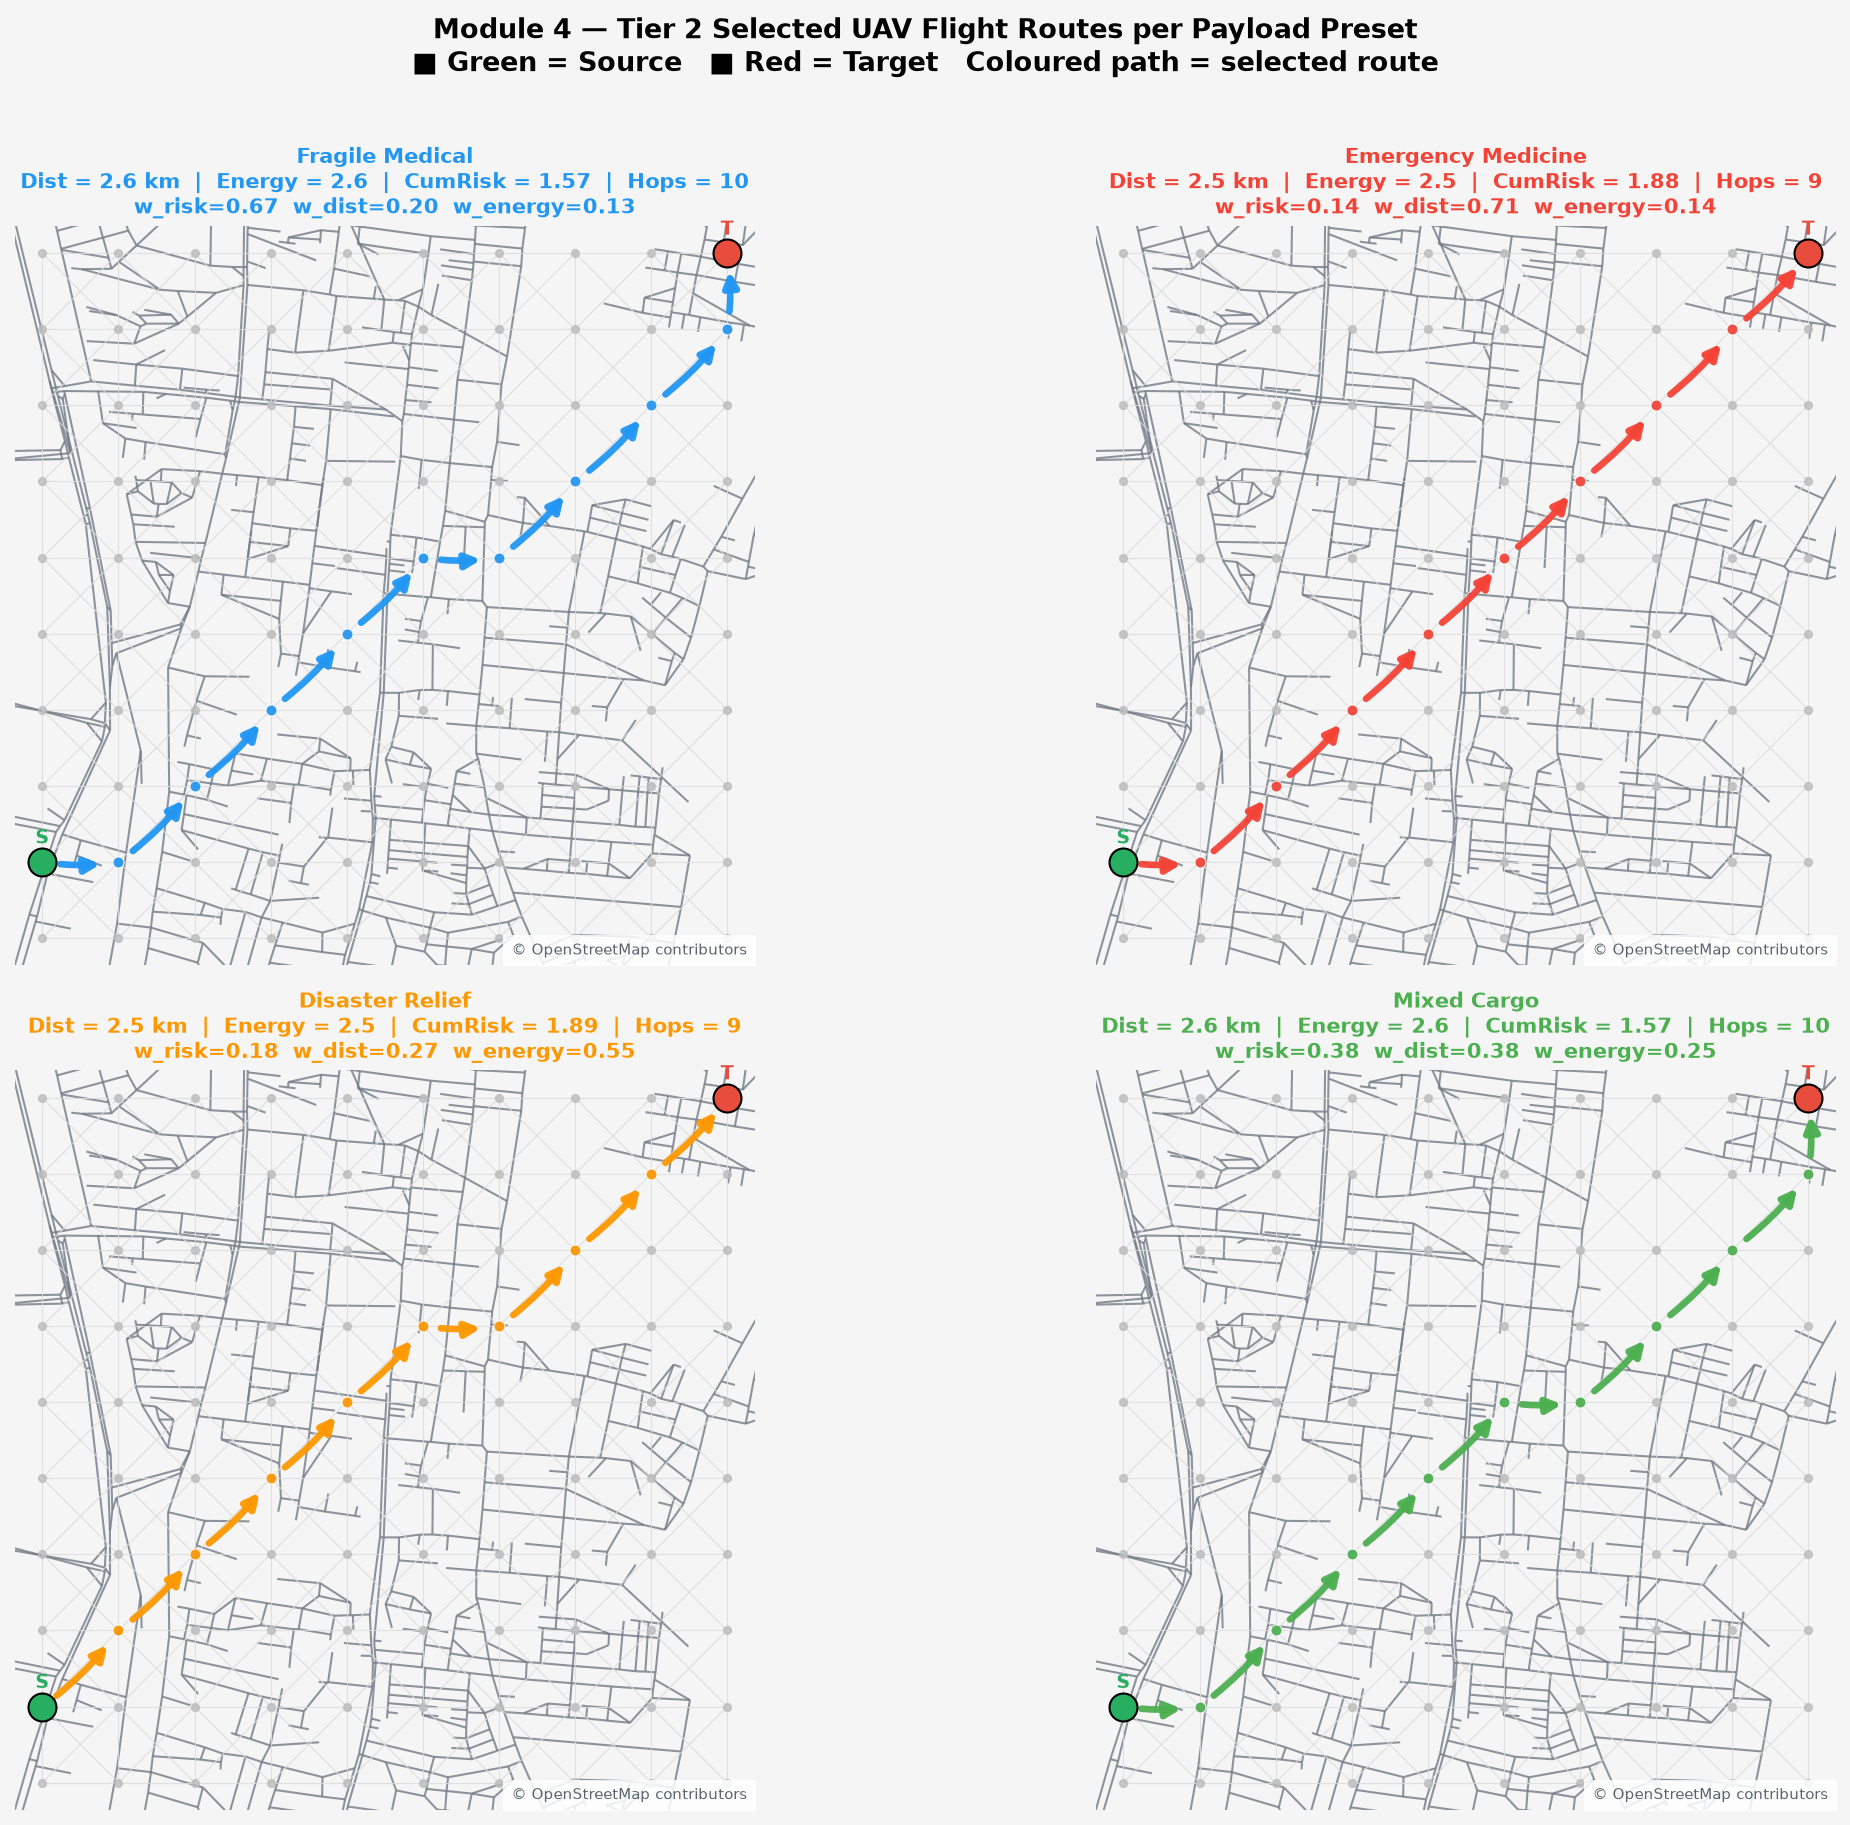
\includegraphics[width=0.48\textwidth]{images/osm_module4_routes_on_graph.jpg}
\caption{Tier~2 routes for the four presets on the 2\,km lattice}\label{fig:osm-routes}
\end{figure}

The first monotonicity check reported 660 violations on the smallest benchmark, but it
had compared selections across scenarios; grouped by scenario, the count is zero.

\subsection{Simulation results}

In E6 the SITL mission runner flew planner missions against ArduCopter SITL. Mission
upload, read-back, the switch to AUTO, the landing and the disarm all succeeded. The
cross-track root-mean-square error between the flown and planned tracks was
0.11--0.13\,m, and the landing offset from the destination pad was 0.01--0.02\,m. These
numbers show that the mission chain from Tier~2 to the autopilot is correct, including
the altitude frame, which is easy to get wrong over uneven terrain.

Figure~\ref{fig:sitl} shows a Tier~2 mission flown in AUTO inside the Gazebo city world,
with the MAVProxy console on the left and the mission in QGroundControl on the right.
The Gazebo world has no wind yet, so logged comparisons across wind cases are planned
for the next pass.

\begin{figure}[!htbp]
\centering
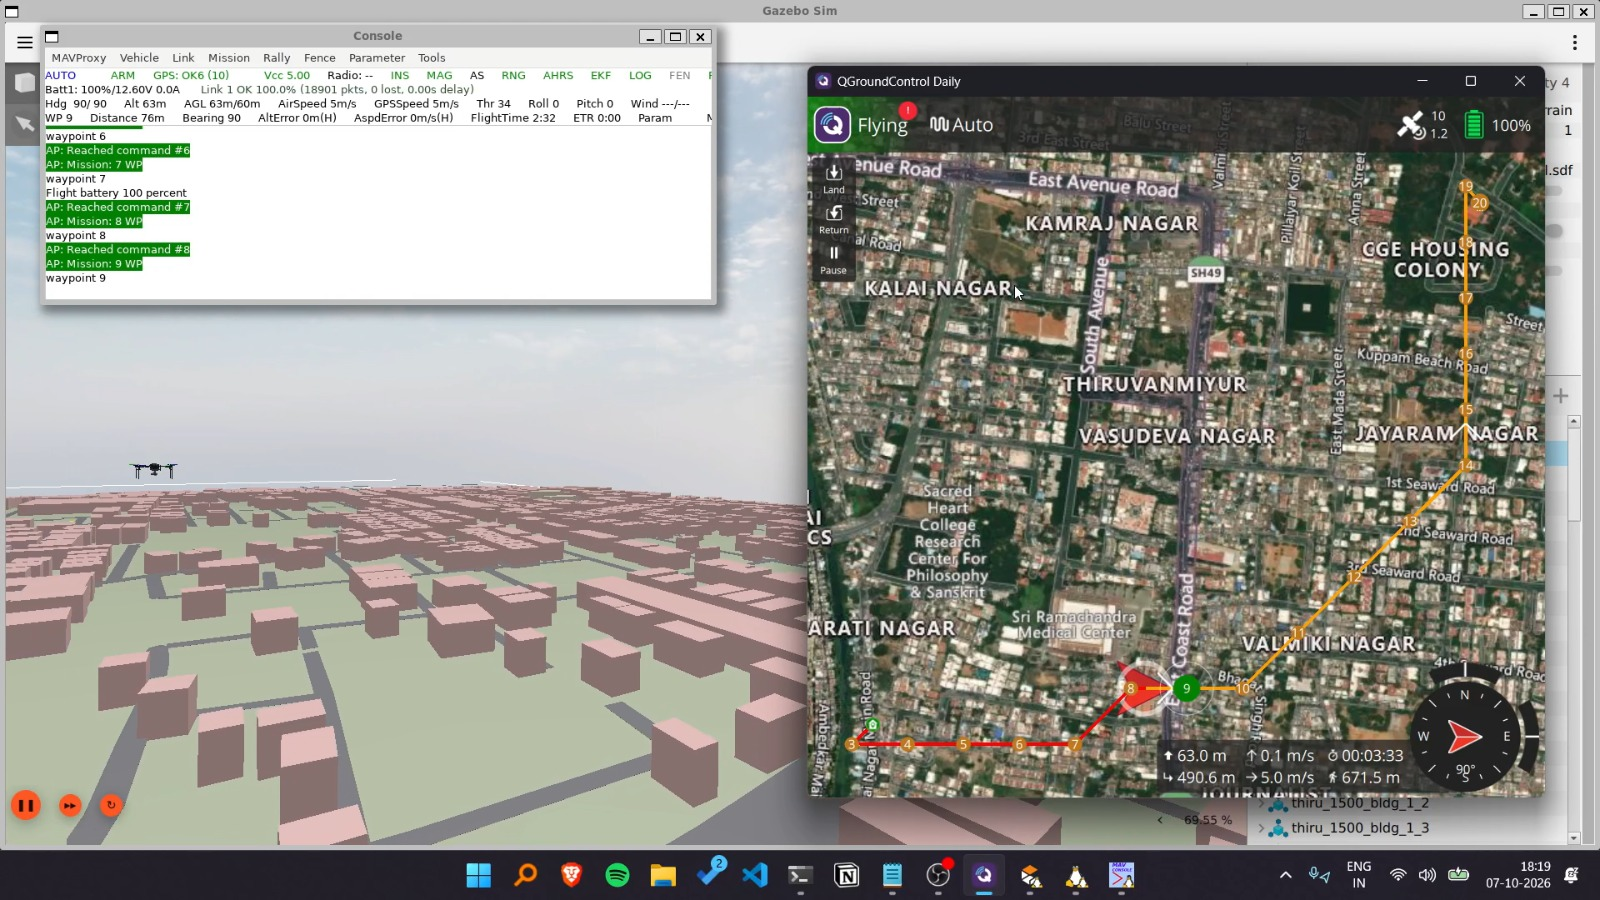
\includegraphics[width=0.6\textwidth]{images/sitl_gazebo_screenshot.jpg}
\caption{Gazebo Harmonic and ArduPilot SITL flying an uploaded Tier~2 mission in AUTO:
MAVProxy console (left), QGroundControl mission view (right)}\label{fig:sitl}
\end{figure}

\subsection{Comparison with existing work}

Table~\ref{tab:compare} compares the system with the planners reviewed in
Chapter~\ref{cha:lit}.

\begin{footnotesize}
\begin{longtable}{|P{1.8cm}|P{2.4cm}|P{2.1cm}|P{2.1cm}|P{2.3cm}|P{2.9cm}|}
\caption{Comparison with the reviewed planners}\label{tab:compare}\\
\hline
\textbf{Property} & \textbf{Chokkalingam and Ganesan~\cite{r1}} & \textbf{Ren et al.~\cite{r3}} & \textbf{Deng et al.~\cite{r11}} & \textbf{Tsoutsouras et al.~\cite{r10}} & \textbf{This work}\\
\hline
\endfirsthead
\hline
\textbf{Property} & \textbf{Chokkalingam and Ganesan~\cite{r1}} & \textbf{Ren et al.~\cite{r3}} & \textbf{Deng et al.~\cite{r11}} & \textbf{Tsoutsouras et al.~\cite{r10}} & \textbf{This work}\\
\hline
\endhead
Front construction & POPSO, stochastic & CDNSGA-II, stochastic & MS-INSGA2, stochastic & None; one trajectory & NAMOA*, exact and deterministic\\
\hline
Objectives & Length, energy, safety, obstacle penalty, weather factor & Distance, safety & Length, collision risk, smoothness & Deadline misses under energy and mass limits & Distance, energy, risk (11 components)\\
\hline
Final route selection & Weighted sum, weights set per mission & Crowding distance ($k$ nearest) & Not discussed & Not applicable & Utility from payload tags, argmax over the full front\\
\hline
Payload in selection & No & No & No & Mass in the power model only & Fragility, weight class, urgency, priority\\
\hline
Wind & Speed-only factor, uniform & Not modelled & Future work & Not modelled & Headwind and crosswind per edge, gust, shear, weather gate\\
\hline
Front reuse & Re-run per mission & Re-run per mission & Re-run per task & Not applicable & Stored front with drift-based refresh\\
\hline
\end{longtable}
\end{footnotesize}

The comparison is qualitative, as their datasets and code are not public; the next pass
scores their selection rules on our fronts (Section~\ref{sec:m5}).
